\chapter{Concept Design}
\label{chap:concept_design}

\section{Introduction}

This chapter presents a detailed outline of the design process for a rotating climbing surface, emphasizing the mechanical design principles integrated with electronic and computer system engineering. The project's primary aim is to design and manufacture a rotating climbing surface capable of providing a facility for extended-duration indoor climbing.

\section{Problem Definition}
\label{sec:problem_definition}

This project aims to develop a rotating climbing surface capable of rotating at a constant, user-defined speed and adjustable incline. The system must exhibit precise control over both speed and incline, as well as incorporate safety measures for user safety.

Key aspects of the project include the design and implementation of robust mechanical and electronic systems to facilitate smooth operation, integrating sensor technologies for accurate speed and inclination detection, and developing an intuitive and simplistic user interface for seamless interaction.

The rotating climbing surface should also adhere to stringent safety guidelines to mitigate potential hazards associated with operation. This encompasses utilizing calculations and simulations to ensure structural integrity, as well as a series of load tests that will need to be passed.

\section{Stakeholder Requirements}

The stakeholder requirements define the intended services of the system and the restrictions on achieving them.

\begin{table}[H]
\centering
\caption{Stakeholder Requirements}
\label{tab:stakeholder-requirements}
\begin{tabular}{|>{\centering\arraybackslash}p{0.1\linewidth}|>{\raggedright\arraybackslash}p{0.15\linewidth}|>{\raggedright\arraybackslash}p{0.55\linewidth}|>{\centering\arraybackslash}p{0.1\linewidth}|}
\hline
\textbf{Number}  & \textbf{Stakeholder} & \textbf{Description} & \textbf{Priority} \\
\hline
SR1  & End-user & Simulate continuous climbing & Must Have \\
SR2  & End-user & Incline adjustment for different difficulty levels & Must Have \\
SR3  & End-user & User-adjustable speed control to accommodate various training intensities & High \\
SR4  & End-user, Safety Officer & Durable and safe construction to withstand continuous use & High \\
SR5  & End-user, Safety Officer & Emergency stop feature for immediate halting of the wall for user safety & Must Have \\
SR6  & End-user & Large enough surface for comfortable climbing experience & High \\
SR7 & Investor, Customer & Affordability & Medium \\
\hline
\end{tabular}
\end{table}

\section{Engineering Requirements}

The stakeholder requirements given in the previous section were expressed by the design team as functional requirements (FRs) in Table \ref{tab:functional-requirements} and performance requirements (PRs) in Table \ref{tab:performance-requirements}. Where relevant, the number of the stakeholder requirement that the engineering requirement was derived from is indicated in the right-hand column. FRs give the actions that the system being designed must do, as seen by the stakeholders. Internal or derived functions are considered in later sections. The PRs are measures of how well the system should perform its functions.

\begin{table}[H]
\centering
\caption{Functional Requirements}
\label{tab:functional-requirements}
\begin{tabular}{|c|p{0.6\linewidth}|>{\centering\arraybackslash}p{0.2\linewidth}|}
\hline
\textbf{FR Number} & \textbf{Description} & \textbf{Related Stakeholder Requirement} \\
\hline
FR1 & Speed control and adjustment & SR1, SR3 \\
FR2 & Incline control and adjustment & SR2 \\
FR3 & Simplistic user interface & SR3, SR5 \\
FR4 & Safety mechanisms & SR5 \\
FR5 & Size compliance & SR6 \\
FR6 & Load compliance & SR6 \\
\hline
\end{tabular}
\end{table}

\begin{table}[H]
\centering
\caption{Performance Requirements}
\label{tab:performance-requirements}
\begin{tabular}{|c|p{0.4\linewidth}|c|c|c|c|}
\hline
\textbf{PR} & \textbf{Description} & \textbf{Target} & \textbf{Range} & \textbf{Unit} & \textbf{Related FR} \\
\hline
PR1 & Maximum rotation speed & 25 & 0--25 & m/min & FR1 \\
PR2 & Maximum negative inclination angle & -45 & -30 to -45 & degrees & FR2 \\
PR3 & Maximum positive inclination angle & +15 & +10 to +20 & degrees & FR2 \\
PR4 & Emergency stop halt time & $<$1 & $<$2 & seconds & FR4 \\
PR5 & Load capacity of climbing wall & 100 & 0--100 & kg & FR6 \\
PR6 & Climbing surface width & 1.5 & 1.4--1.6 & m & FR5 \\
PR7 & Climbing surface height & 2.9 & 2.5--3.1 & m & FR5 \\
\hline
\end{tabular}
\end{table}

\section{Subsystem Identification and Selection}
\label{sec:concept_selection}

Based on the specified requirements and specifications of the rotating climbing surface, several key subsystems are crucial for the design and implementation of the system.

\subsection{Subsystem Identification}

\begin{enumerate}
    \item \textbf{Inclination Adjustment System:} Allows the inclination of the rotating climbing surface to be adjusted to vary difficulty levels.
    \item \textbf{Braking System:} Responsible for controlling the rate of rotation, thus controlling the speed of the climbing surface. The speed should be constant and smooth.
    \item \textbf{Rotating Surface:} The physical surface that rotates, allowing climbing holds to be mounted on it.
    \item \textbf{Control System and User Interface:} Serves as the connection between the user's preferences and the control of inclination and speed. It must be intuitive and user-friendly, enabling clear adjustment control over the necessary parameters.
    \item \textbf{Safety System:} Able to cut power to all high-power electronics and allow rotation to come to a rapid stop as soon as the emergency stop button is activated. The system should also ensure that all electronics and moving parts are enclosed.
\end{enumerate}

\subsection{Functional Decomposition}

The functional requirements detailed previously outline the actions the rotating climbing wall system must perform from the stakeholders' perspective. In this section, these requirements are further decomposed to identify the internal functions the system must execute. Figure~\ref{fig:functional-decomp} illustrates the flow of energy, information, and materials to and from the functions that consume, generate, or transform these flows within the rotating climbing wall system.

\begin{figure}[H]
    \centering
    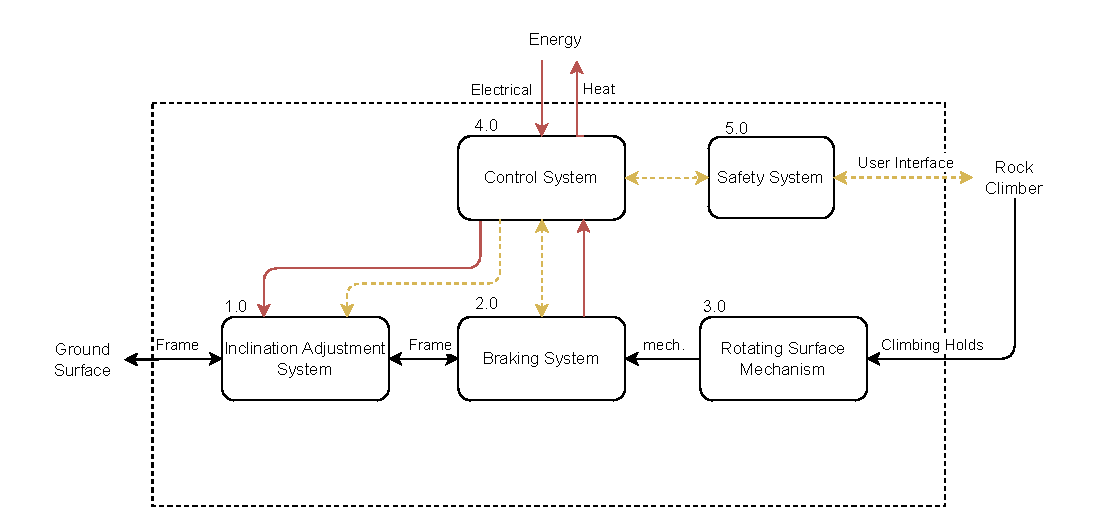
\includegraphics[width=1\linewidth]{figs/concept_design/Functional_Decomp_Flow.pdf}
    \caption{Top-Level Functional Decomposition}
    \label{fig:functional-decomp}
\end{figure}

\section{Concept Development}

\subsection{Inclination Adjustment System}

\subsubsection{Introduction}

The inclination adjustment system allows for altering the climbing angle of the wall, making it more beginner-friendly with less steep angles or more challenging with overhangs for advanced climbers and intense training sessions. This subsystem addresses FR2 (Incline control and adjustment) and PR2 and PR3 from the performance requirements.

\subsubsection{Concept Generation}

\paragraph{IAS1: Linear Actuation}

This concept uses linear actuators connected to the frame of the climbing wall to adjust its angle. The actuators can be controlled electronically, allowing for precise and automated inclination adjustments through a user interface.

\begin{figure}[H]
    \centering
    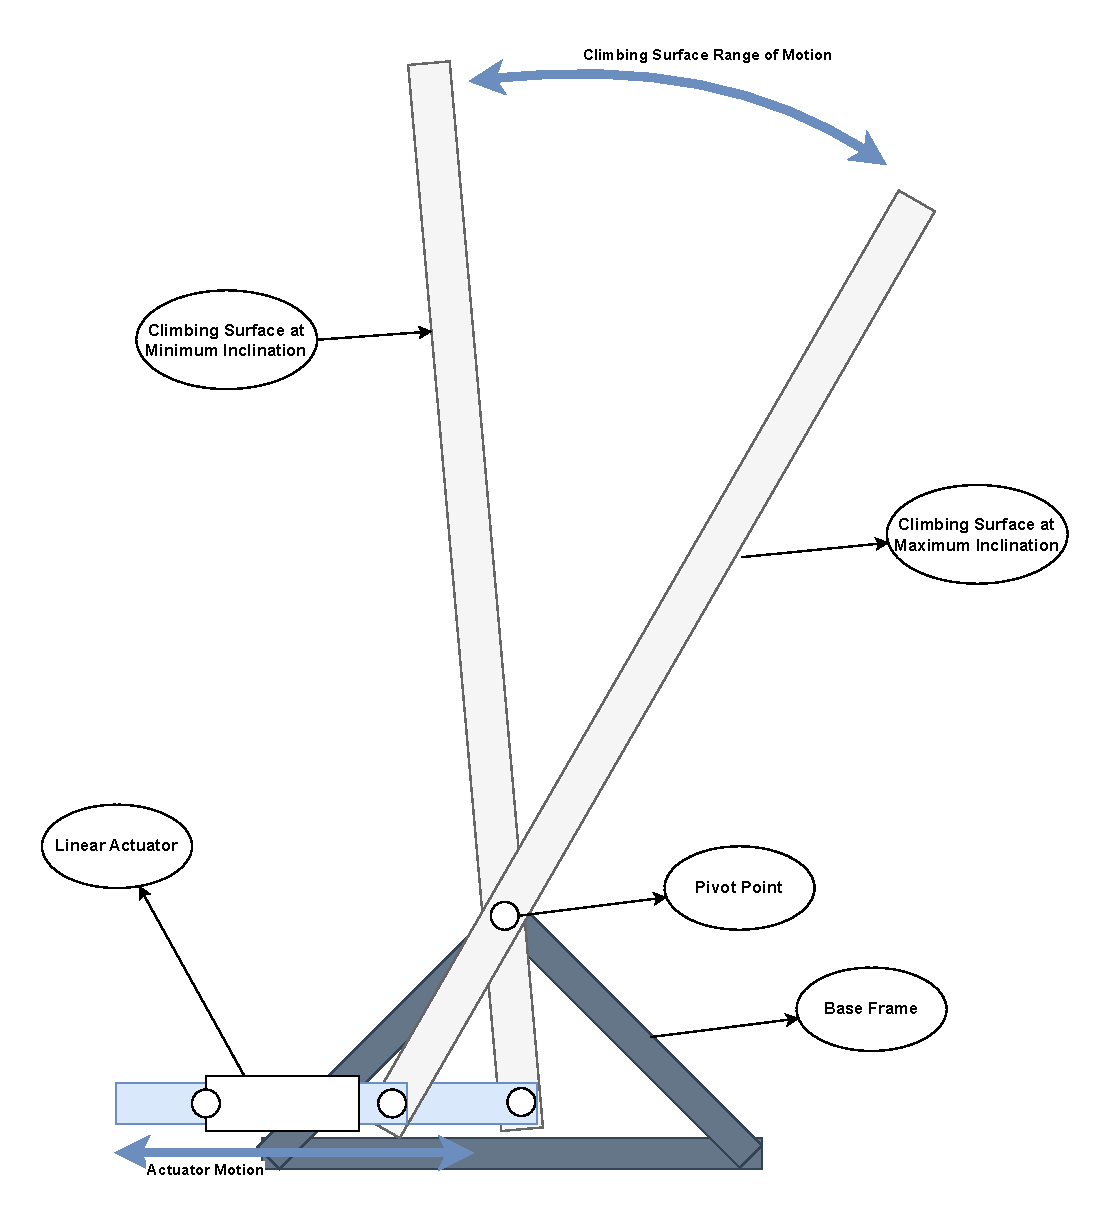
\includegraphics[width=0.6\linewidth]{figs/concept_design/Linear_Actuator_Concept.pdf}
    \caption{Linear Actuator Concept Sketch}
    \label{fig:linear-actuator-concept}
\end{figure}

\textbf{Advantages:}
\begin{itemize}
    \item Precise and automated control over inclination.
    \item Smooth operation with electronic integration.
    \item Can be integrated with safety mechanisms.
\end{itemize}

\textbf{Disadvantages:}
\begin{itemize}
    \item Higher cost due to actuators and control systems.
    \item Increased complexity in design and maintenance.
\end{itemize}

\paragraph{IAS2: Hand-Crank Inclination}

This manual method employs a hand-crank mechanism connected to the wall's support structure, allowing users to adjust the inclination manually.

\begin{figure}[H]
    \centering
    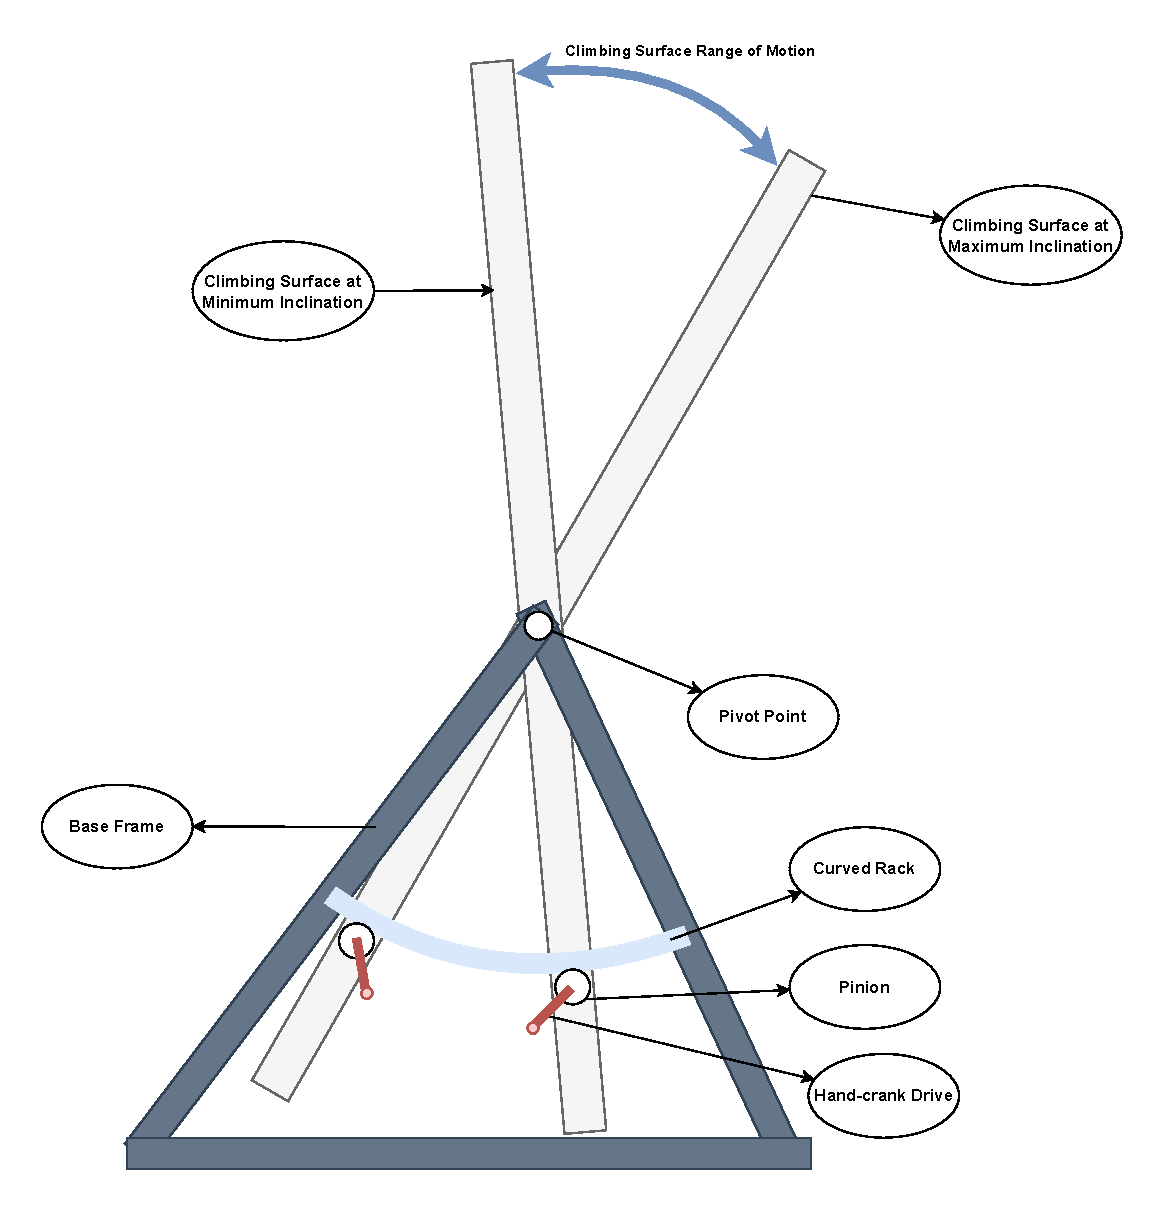
\includegraphics[width=0.6\linewidth]{figs/concept_design/Handcrank_Concept.pdf}
    \caption{Hand-Crank Inclination Concept Sketch}
    \label{fig:handcrank-concept}
\end{figure}

\textbf{Advantages:}
\begin{itemize}
    \item Low cost and simplicity.
    \item Minimal electronic components, reducing potential failures.
\end{itemize}

\textbf{Disadvantages:}
\begin{itemize}
    \item Requires manual effort, which may be inconvenient.
    \item Lacks precision and may need additional mechanisms to secure the angle.
    \item Safety concerns if not properly locked in place.
\end{itemize}

\paragraph{IAS3: Worm Gear Automatic Inclination}

This concept uses a motor-driven worm gear mechanism to adjust the inclination. The worm gear provides self-locking capabilities, preventing unintended movement, and allows for precise electronic control.

\begin{figure}[H]
    \centering
    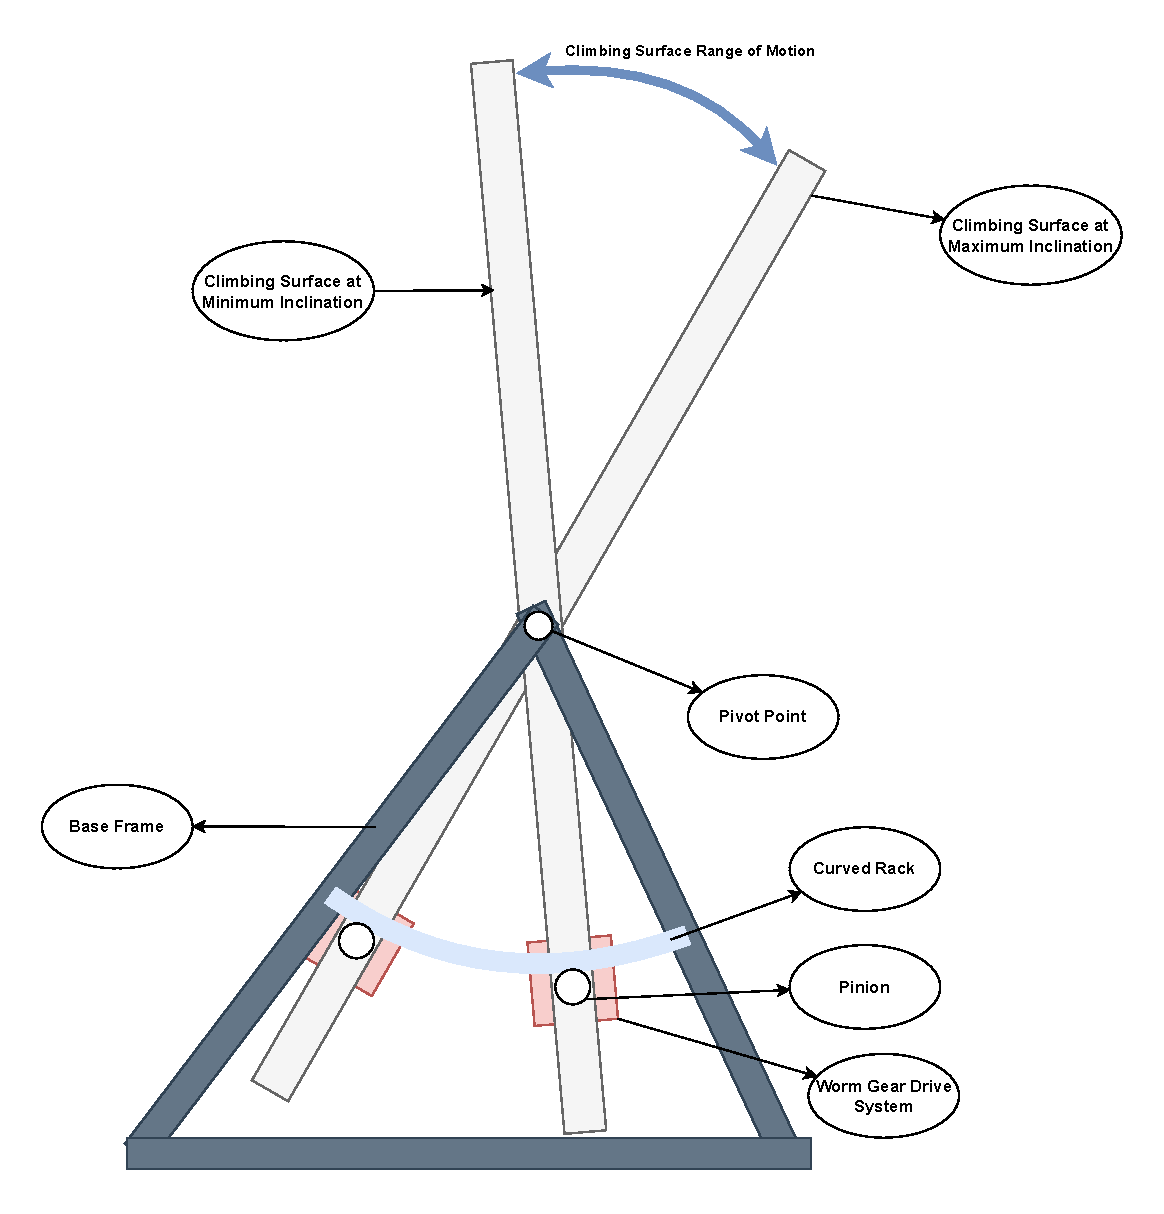
\includegraphics[width=0.6\linewidth]{figs/concept_design/WormGear_Concept.pdf}
    \caption{Worm Gear Automatic Inclination Concept Sketch}
    \label{fig:wormgear-concept}
\end{figure}

\textbf{Advantages:}
\begin{itemize}
    \item Precise control with electronic integration.
    \item Self-locking mechanism enhances safety.
    \item Durable and reliable over long-term use.
\end{itemize}

\textbf{Disadvantages:}
\begin{itemize}
    \item Moderate cost due to mechanical components and motor.
    \item Increased complexity compared to manual systems.
\end{itemize}

\subsubsection{Concept Evaluation and Selection}

\paragraph{Selection Criteria}

\begin{enumerate}
    \item Ease of Operation (Weight: 1)
    \item Cost (Weight: 2)
    \item Complexity (Weight: 2)
    \item Safety Mechanisms (Weight: 3)
    \item Reliability (Weight: 2)
    \item Range of Motion (Weight: 1)
    \item Maintenance Requirement (Weight: 1)
\end{enumerate}

\paragraph{Decision Matrix}

\begin{table}[H]
\centering
\caption{Inclination Adjustment System Decision Matrix}
\label{tab:ias_decision_matrix}
\begin{tabular}{|p{0.1\linewidth}|p{0.3\linewidth}|c|c|c|}
\hline
\textbf{Criterion} & \textbf{Description} & \textbf{IAS1} & \textbf{IAS2} & \textbf{IAS3} \\
\hline
Ease of Operation (1) & User effort required to adjust inclination & +1 & -1 & +1 \\
\hline
Cost (2) & Total cost of implementation & -1 & +1 & 0 \\
\hline
Complexity (2) & Complexity of design and implementation & -1 & +1 & 0 \\
\hline
Safety Mechanisms (3) & Ability to prevent unintended movement & +1 & -1 & +1 \\
\hline
Reliability (2) & Likelihood of consistent performance over time & 0 & +1 & +1 \\
\hline
Range of Motion (1) & Ability to achieve desired angles & +1 & -1 & +1 \\
\hline
Maintenance Requirement (1) & Frequency and difficulty of maintenance & +1 & -1 & +1 \\
\hline
\textbf{Weighted Total} &  & \textbf{+4} & \textbf{-1} & \textbf{+8} \\
\hline
\end{tabular}
\end{table}

\paragraph{Selection Justification}

Based on the weighted totals, IAS3 (Worm Gear Automatic Inclination) is the preferred concept. It offers precise control, inherent safety due to its self-locking mechanism, and high reliability, all of which are critical for the system's performance and user safety.

\subsection{Braking System}

\subsubsection{Introduction}

The braking system is responsible for controlling the rate of rotation, ensuring the climbing surface moves at a constant and smooth speed. This subsystem addresses FR1 (Speed control and adjustment) and PR1 from the performance requirements.

\subsubsection{Concept Generation}

\paragraph{BS1: Hydraulic Braking System}

This concept uses a hydraulic motor/pump operating in reverse to provide resistance against the rotation. The hydraulic fluid flows through a manually adjustable flow control valve, such as a needle valve, to regulate the speed.

\begin{figure}[H]
    \centering
    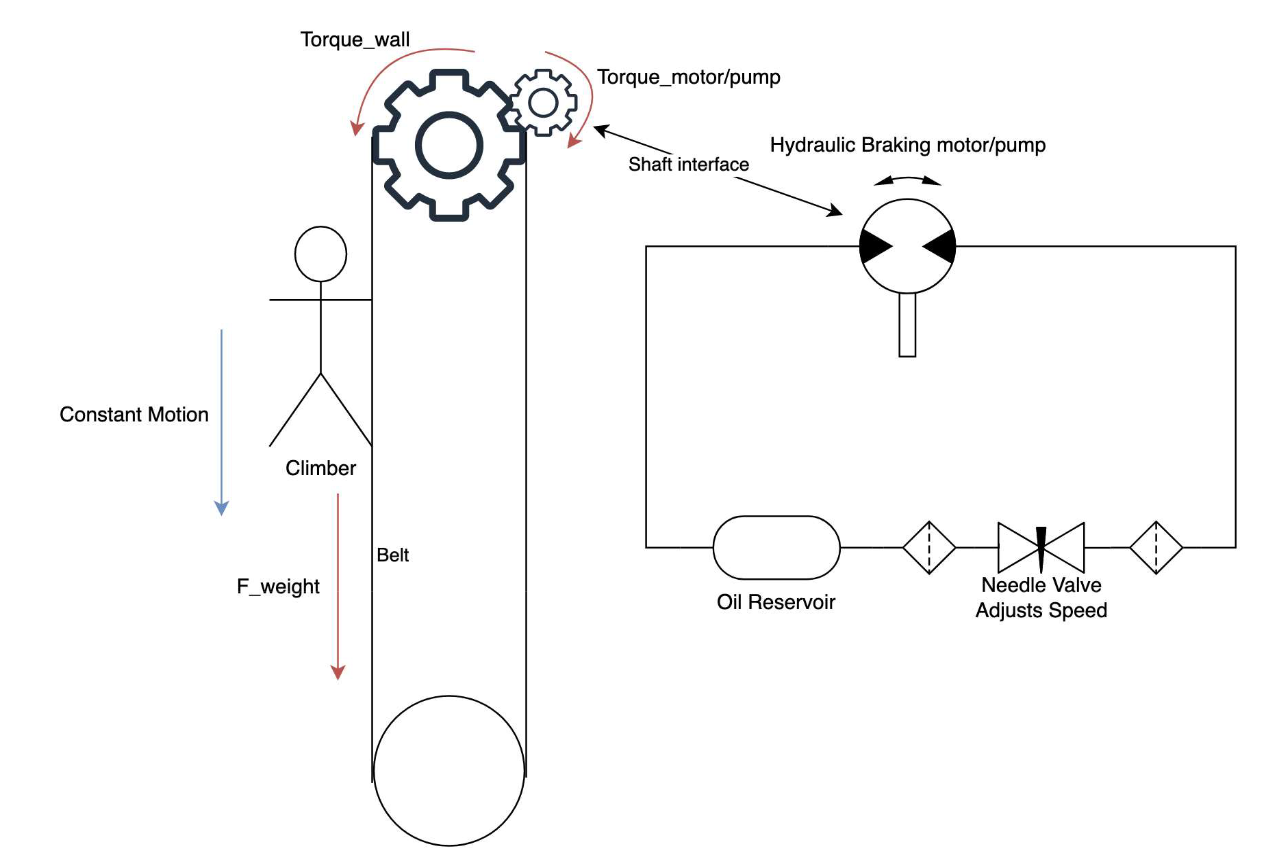
\includegraphics[width=0.6\linewidth]{figs/concept_design/hydraulic_brake_concept.png}
    \caption{Hydraulic Braking System Concept Sketch}
    \label{fig:hydraulic-brake-concept}
\end{figure}

\textbf{Advantages:}
\begin{itemize}
    \item Simple mechanical system without electronic controls.
    \item Robust and durable components.
\end{itemize}

\textbf{Disadvantages:}
\begin{itemize}
    \item Lacks precise electronic control.
    \item Manual adjustments required for speed changes.
    \item Potential for leaks and maintenance issues.
\end{itemize}

\paragraph{BS2: Disk Braking System}

This concept adapts an off-the-shelf disk brake system from a motorcycle or mountain bike, controlled automatically to maintain constant rotational speed. Sensors monitor the current speed, and a PID controller adjusts the brake caliper to achieve the desired speed.


\textbf{Advantages:}
\begin{itemize}
    \item Inexpensive and straightforward design.
    \item Utilizes readily available components.
\end{itemize}

\textbf{Disadvantages:}
\begin{itemize}
    \item Potential overheating of brake pads and disk due to continuous use.
    \item Wear and tear leading to frequent maintenance.
    \item Limited precision in speed control.
\end{itemize}

\textbf{Heat Analysis:}

A lumped sum analysis and heat simulation in Fusion 360 were performed to evaluate the thermal performance of the disk brake system. The results indicated that the brake pads and disk would reach unsafe temperatures after extended use, compromising safety and functionality. This thermal limitation makes BS2 unsuitable for continuous operation required in this application.

\paragraph{BS3: Electromagnetic Braking System}

This concept uses an electric motor and driver to provide electromagnetic braking. The system employs a braking resistor to dissipate the energy generated by the climber-induced rotation.


\textbf{Advantages:}
\begin{itemize}
    \item Precise electronic control over speed.
    \item Smooth and consistent braking performance.
    \item Low maintenance with no physical contact components.
\end{itemize}

\textbf{Disadvantages:}
\begin{itemize}
    \item Higher initial cost due to motor and control systems.
    \item Requires electrical expertise for implementation.
\end{itemize}

\subsubsection{Concept Evaluation and Selection}

\paragraph{Selection Criteria}

\begin{enumerate}
    \item Ease of Integration (Weight: 2)
    \item Cost (Weight: 3)
    \item Maintenance Requirement (Weight: 2)
    \item Precision of Control (Weight: 3)
    \item Safety (Weight: 3)
    \item Reliability (Weight: 2)
\end{enumerate}

\paragraph{Decision Matrix}

\begin{table}[H]
\centering
\caption{Braking System Decision Matrix}
\label{tab:bs_decision_matrix}
\begin{tabular}{|p{0.1\linewidth}|p{0.3\linewidth}|c|c|c|}
\hline
\textbf{Criterion} & \textbf{Description} & \textbf{BS1} & \textbf{BS2} & \textbf{BS3} \\
\hline
Ease of Integration (2) & Complexity of integrating into system & 0 & +1 & +1 \\
\hline
Cost (3) & Total cost of implementation & -1 & +1 & -1 \\
\hline
Maintenance Requirement (2) & Frequency and difficulty of maintenance & -1 & -1 & +1 \\
\hline
Precision of Control (3) & Ability to precisely control speed & -1 & 0 & +1 \\
\hline
Safety (3) & Safety considerations during operation & 0 & -1 & +1 \\
\hline
Reliability (2) & Likelihood of consistent performance over time & +1 & -1 & +1 \\
\hline
\textbf{Weighted Total} &  & \textbf{-2} & \textbf{0} & \textbf{+8} \\
\hline
\end{tabular}
\end{table}

\paragraph{Selection Justification}

BS3 (Electromagnetic Braking System) is the preferred concept based on the weighted total. It offers precise control, high safety, low maintenance, and reliability, which are critical factors for the braking system. The higher initial cost is justified by the long-term benefits and performance.

\subsection{Rotating Surface}

\subsubsection{Introduction}

The rotating surface is the central component of the system, providing the physical structure on which climbers ascend. It must securely hold climbing holds and rotate smoothly under load. This subsystem addresses FR5 (Size compliance) and FR6 (Load compliance), along with PR5, PR6, and PR7 from the performance requirements.

\subsubsection{Concept Generation}

\paragraph{RS1: Conveyor Chain-Driven Panels}

This concept uses a series of interconnected panels attached to conveyor chains on either side. The chains are looped over sprockets at the top and bottom, driven by the main shafts. The panels form the climbing surface and are pulled along by the chains.


\textbf{Advantages:}
\begin{itemize}
    \item Strong and robust connection between panels and drive system.
    \item Capable of handling high loads from climbers.
    \item Reliable operation with well-understood technology.
\end{itemize}

\textbf{Disadvantages:}
\begin{itemize}
    \item Higher cost due to chains and sprockets.
    \item Increased weight of the system.
    \item Requires precise alignment to prevent chain derailment.
\end{itemize}

\paragraph{RS2: Rubber Conveyor Belt Panels}

This concept employs a continuous rubber conveyor belt with climbing holds attached directly to the belt or to panels affixed to the belt. The belt wraps around drums or rollers at the top and bottom, driven by the main shafts.

\textbf{Advantages:}
\begin{itemize}
    \item Simpler construction with fewer moving parts.
    \item Potentially lower cost than chain systems.
    \item Smooth and continuous climbing surface.
\end{itemize}

\textbf{Disadvantages:}
\begin{itemize}
    \item Limited load capacity; may not handle high loads well.
    \item Difficulty in attaching and securing climbing holds.
    \item Potential for belt stretching and slippage over time.
\end{itemize}

\subsubsection{Concept Evaluation and Selection}

\paragraph{Selection Criteria}

\begin{enumerate}
    \item Load Capacity (Weight: 3)
    \item Durability (Weight: 2)
    \item Cost (Weight: 2)
    \item Ease of Maintenance (Weight: 1)
    \item Surface Quality (Weight: 2)
    \item Complexity of Construction (Weight: 1)
\end{enumerate}

\paragraph{Decision Matrix}

\begin{table}[H]
\centering
\caption{Rotating Surface Decision Matrix}
\label{tab:rs_decision_matrix}
\begin{tabular}{|p{0.1\linewidth}|p{0.3\linewidth}|c|c|}
\hline
\textbf{Criterion} & \textbf{Description} & \textbf{RS1} & \textbf{RS2} \\
\hline
Load Capacity (3) & Ability to support climber weight & +1 & -1 \\
\hline
Durability (2) & Resistance to wear and tear & +1 & 0 \\
\hline
Cost (2) & Total cost of implementation & -1 & +1 \\
\hline
Ease of Maintenance (1) & Frequency and difficulty of maintenance & 0 & +1 \\
\hline
Surface Quality (2) & Smoothness and suitability for climbing & +1 & +1 \\
\hline
Complexity of Construction (1) & Difficulty in manufacturing and assembly & -1 & +1 \\
\hline
\textbf{Weighted Total} &  & \textbf{+5} & \textbf{+2} \\
\hline
\end{tabular}
\end{table}

\paragraph{Selection Justification}

RS1 (Conveyor Chain-Driven Panels) is the preferred concept due to its superior load capacity and durability, which are essential for supporting climbers safely. While it has higher costs and complexity, these drawbacks are offset by the benefits in performance and safety.

\section{Integration of Subsystems}

The selected concepts for each subsystem are designed to work cohesively within the overall system. The frame structure integrates the inclination adjustment system, braking system, and rotating surface. The frame must accommodate the dimensions specified (PR6 and PR7) and provide mounting points for the mechanical components.

\subsection{Frame Structure}

The frame is constructed using steel beams sized according to the chosen dimensions (approximately 1.6\,m width and 2.9\,m height). All shaft widths, upright beams, crossbeams, and other structural components are designed based on these dimensions. Finite Element Analysis (FEA) will be conducted to ensure structural integrity under the expected loads.

\section{Conclusion}

Through a rigorous concept development and evaluation process, the preferred concepts for each of the main subsystems have been selected:

\begin{itemize}
    \item \textbf{Inclination Adjustment System:} IAS3 (Worm Gear Automatic Inclination)
    \item \textbf{Braking System:} BS3 (Electromagnetic Braking System)
    \item \textbf{Rotating Surface:} RS1 (Conveyor Chain-Driven Panels)
\end{itemize}

These selections are justified based on their performance against the defined criteria, alignment with stakeholder and engineering requirements, and their ability to integrate effectively within the overall system design.

Future work will focus on detailed design, including precise calculations, simulations, and integration of the control and safety systems.

